%14_binary_tree.tex
%notes for the course PandA1 COMS10002 taught at the University of Bristol
%2017 Conor Houghton conor.houghton@bristol.ac.uk

%To the extent possible under law, the author has dedicated all copyright 
%and related and neighboring rights to these notes to the public domain 
%worldwide. These notes are distributed without any warranty. 

\documentclass[11pt,a4paper]{scrartcl}
\typearea{12}
\usepackage{graphicx}
\usepackage{pstricks}
\usepackage{listings}
\usepackage{tikz-qtree}
\lstset{language=C}
\pagestyle{headings}
\markright{COMS10001 - PandA2 14\_binary\_tree - Conor}

\tikzset{every tree node/.style={minimum width=2em,draw,circle},
         blank/.style={draw=none},
         edge from parent/.style=
         {draw,->, edge from parent path={(\tikzparentnode) -- (\tikzchildnode)}},
         level distance=1.5cm}

\begin{document}

\subsection*{14 - binary trees\footnote{\texttt{http://github.com/conorhoughton/COMS10001}}}

A binary tree is a data structure somewhat similar to a linked list
except each node leads on to up to two other node, rather than just
one. With the restriction that there are no loops, it can be thought
of as looking something like a tree. The equivalent of the head, the
node that has no other node pointing to it, is called the {\sl root},
but, confusingly, it is very common to put it at the top in
diagrams. Another confusing thing is that a family tree metaphor is
often used, so you talk about a node's {\sl children} or its {\sl
  descendents}, but the botanical expressions root and {\sl leaf}, a
leaf is a childless node. An example binary tree is shown in
Fig.~\ref{fig_example_tree} and code for a node and for making a node,
including the root, is given in Table~\ref{c_node} and
Table~\ref{c_make}.

\begin{figure}
\begin{center}
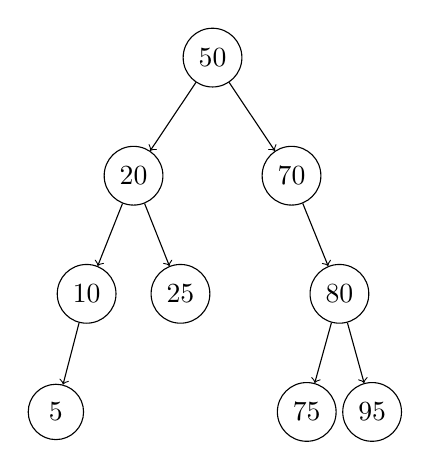
\begin{tikzpicture}
\Tree
[.50     
    [.20 
      [.10
      \edge[]; {5}
      \edge[blank]; \node[blank]{};
      ]
      \edge[]; {25}
    ]
    [.70  
    \edge[blank]; \node[blank]{};
    \edge[]; [.80
                \edge[]; {75}
                \edge[]; {95}
              ]
    ]
]
\end{tikzpicture}
\end{center}
\caption{An example binary tree. The node containing 50 is the root; the nodes containing 50, 20 and 80 have two children, the nodes with 25, 75 and 95 have no descendents, the node with 10 only has a left child, the one with 70 only has a right child.\label{fig_example_tree}}
\end{figure}


\begin{table}
\begin{lstlisting}[numbers=left]
struct node
{
  int entry;
  struct node *left;
  struct node *right;
};
\end{lstlisting}
\caption{A node, it has a variable to store the entry and pointers to the left and right children. \label{c_node}}
\end{table}


\begin{table}
\begin{lstlisting}[numbers=left]
struct node * make_node(int new_entry)
{
  struct node * a_node=(struct node *)malloc(sizeof(struct node));
  a_node->entry=new_entry;

  a_node->left=NULL;
  a_node->right=NULL;

  return a_node;
}
\end{lstlisting}
\caption{Functions for making a node. \label{c_make}}
\end{table}


The most common application for a binary tree as a data structure is
the binary search tree. In a binary search tree the nodes are arranged
so that a node's left child has a smaller value and its right child a
greater one. This makes searching easy, you start at the root and at
each node go left of right according to whether the value you are
search for is bigger or smaller than the node value. For this to work
the nodes must be added the same way, so that a left child is always
smaller and a right child bigger; doing this is easy, basically you
act as if you were searching for the entry you wish to add and if the
next place you want to look is a NULL, you add the node there. There
is code for adding a node at Table~\ref{c_add} and for finding a node
at Table~\ref{c_find}.


\begin{table}
\begin{lstlisting}[numbers=left]
struct node * add_node(struct node * here,int new_entry)
{

  if(here==NULL)
    return make_node(new_entry);

  if(new_entry<here->entry)
      here->left = add_node(here->left,new_entry);
  else
      here->right = add_node(here->right,new_entry);
  return here;

}
\end{lstlisting}
\caption{Adds a node. This is done recursively, searching to the left
  or right until it gets to NULL and making a new node there. See how
  cleverly it does the recursion, it links the current node to the
  return value and then returns itself unless it is NULL, in which
  case it returns the new node.\label{c_add}}
\end{table}


\begin{table}
\begin{lstlisting}[numbers=left]
struct node * find_entry(struct node * root, int a_entry)
{
  if(root==NULL)
    return root;
  else if(root->entry==a_entry)
    return root;

  if(root->entry>a_entry)
    return find_entry(root->left,a_entry);
  return find_entry(root->right,a_entry);
}
\end{lstlisting}
\caption{Finds a node. This is done recursively down the tree and returns a pointer to the node containing the entry, or a NULL pointer if the entry isn't found.\label{c_find}}
\end{table}

As for computational complexity; this depends on how balanced the tree
is. Imagine the tree is balanced, so at each node the number of left
descendents is roughly equal to the number of right descendents. Now,
consider finding; the run time is
\begin{equation}
T_n=c+T_{n/2}
\end{equation}
since at each node you either go left or right, roughly halving the
number of nodes still under consideration. Hence
\begin{equation}
T_n\in O(\log n)
\end{equation}
Making a node is the same, to make a node you first find its position
and then add it, adding it is $O(1)$ so making is $O(\log{n})$.

One way to think about this is to note that when finding you only pass
through each level once, where a level is made up of all the nodes the
same number of nodes away from the root. How many levels are there?
Well, imagine labelling all the nodes with a binary number describing
its position, so you have a node numbered $x$ its left node is $x0$
and its right node is $x1$. To get to the node you would start at the
root and look at the first bit, if it zero you go to the left node, if
it is one, you go to the right node. An example is given in
Fig.~\ref{fig_tree_route}. Now, if all the nodes are packed in
together so there are no wasted labels then the longest words are
about $\log{(n+1)/2}$ bits long. Roughly speaking, this is because
about half the nodes are on the lowest level. Thus the number of
levels, and hence the number of algorithmic steps goes like $\log{n}$.

\begin{figure}
\begin{center}
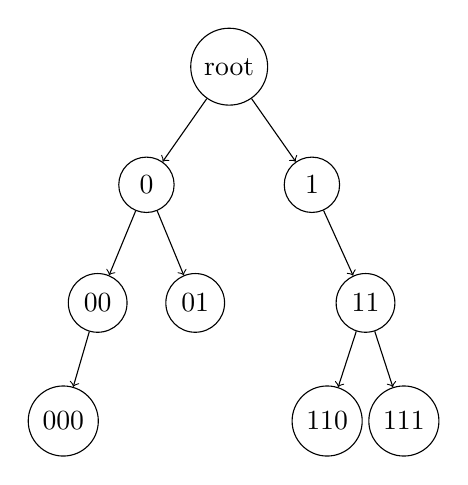
\begin{tikzpicture}
\Tree
[.root
    [.0 
      [.00
      \edge[]; {000}
      \edge[blank]; \node[blank]{};
      ]
      \edge[]; {01}
    ]
    [.1  
    \edge[blank]; \node[blank]{};
    \edge[]; [.11
                \edge[]; {110}
                \edge[]; {111}
              ]
    ]
]
\end{tikzpicture}
\end{center}
\caption{A route map. Here the nodes are labelled in a way that describes their position, starting with the root a 0 indicates a left turn and a 1 a right turn.\label{fig_tree_route}}
\end{figure}

Of course, all this depends on the tree being balanced. This is an
important issue. In Fig.~\ref{fig_balance} we see the tree
corresponding to 10, 20, 25, 30, 35, 40, 45, 50 and the tree
corresponding to the same sequence added in a different order 30, 20,
40, 10, 25, 35, 45. Obviously this would have a big impact on search
times. In fact, we'll see there is a way to balance the trees as the
nodes are added.

\begin{figure}
\begin{center}
\begin{tikzpicture}
\Tree
[.10
  \edge[blank]; \node[blank]{};
  [.20
    \edge[blank]; \node[blank]{};
    [.25
      \edge[blank]; \node[blank]{};
      [.30
          \edge[blank]; \node[blank]{};
          [.35
              \edge[blank]; \node[blank]{};
              [.40
                  \edge[blank]; \node[blank]{};
                  \edge[]; {45}
              ]
          ]
      ]
    ]
  ]
]
\end{tikzpicture}
\qquad
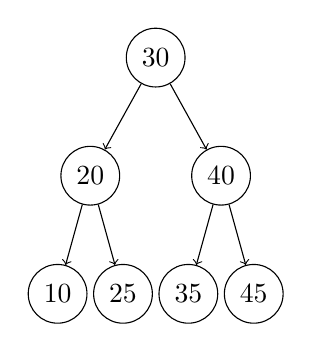
\begin{tikzpicture}
\Tree
[.30
  [.20
    \edge[]; {10}
    \edge[]; {25}
  ]
  [.40
    \edge[]; {35}
    \edge[]; {45}
  ]
]
\end{tikzpicture}
\end{center}
\caption{Trees for the same data. LEFT: Unbalanced tree, seven levels. RIGHT: Balanced tree, three levels.\label{fig_balance}}
\end{figure}

\end{document}
